\subsection{SLIDING TOKENS RECONFIGURATION}

\begin{frame}{SLIDING TOKENS RECONFIGURATION}
\begin{block}{The SLIDING TOKENS problem} 
    \begin{flushleft}
      \textbf{Input Instance: } Two independent sets $I_1$ and $I_2$ of a graph $G = (V,E)$ s.t $|I_1| = |I_2|$ with a token placed on each vertex in $I_1$. \\
      \hfill \break
      \textbf{Question: } Is there a reconfiguration sequence from $I_1$ to $I_2$ ?\\
    \end{flushleft}
   \end{block}
   
   \begin{figure}
        \centering
        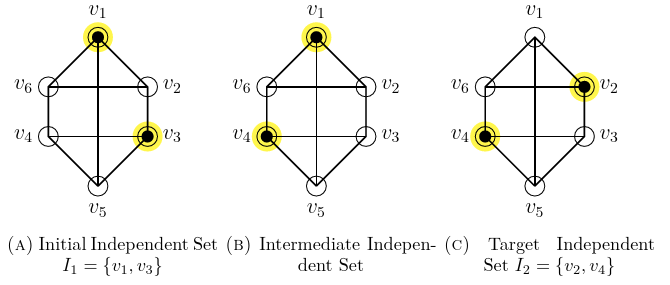
\includegraphics[scale=0.3]{img/sliding.png}
        \caption{Reconfiguration sequence from $I_1$ and $I_2$.}
        \label{fig:ps}
    \end{figure}
\end{frame}

\begin{frame}{SLIDING TOKENS RECONFIGURATION}
    
    Seen as the reconfiguration version of the Independent Set problem.
    
    \begin{block}{Theorem (E.Demaine \& R.Hearn)} The SLIDING TOKENS problem is PSPACE-complete \cite{hearn_demaine_ncl_book}. 
   \end{block}
\end{frame}

\begin{frame}{LABELLED SLIDING TOKENS}
    \begin{block}{The LABELLED SLIDING TOKENS problem}
        \begin{flushleft}
          \textbf{Input Instance: } Two independent sets $I_1$ and $I_2$ of a graph $G = (V,E)$ s.t $|I_1| = |I_2|$ with a labelled token placed on each each vertex in $I_1$ and each label is unique. \\
        \end{flushleft}
    \end{block}    
    
    \begin{block}{Theorem} The LABELLED SLIDING TOKENS problem is PSPACE-complete. 
   \end{block}
   
   \begin{proof} Reduction from the Nondeterministic Constraint Logic.
   \end{proof}
\end{frame}

\begin{frame}{Nondeterministic Constraint Logic}
    \begin{block}{Graph formulation}
    The computational model is a constraint graph $G = (V,E)$ \\ where :
     \begin{itemize}
        \item Each edge is assigned a weight. 
        \item Each vertex has a minimum inflow constraint.
        \item A configuration $=$ orientation of the edges. 
    \end{itemize}
    \end{block}
\end{frame}

\begin{frame}{Nondeterministic Constraint Logic}
  \begin{columns}
    \begin{column}{0.6\textwidth}
    \begin{block}{Restricted NCL}
    The constraint graph $G = (V, E)$
      \begin{itemize}
        \item $3$-regular.
        \item Uses only weights $\in \{1,2\}$ \\ 
        Red and blue edges.
        \item Uses only two types of vertices \\ 
        AND and OR vertices. 
        \item The minimum inflow constraint $ = 2$.
      \end{itemize}
   \end{block}
   \end{column}
   
   \begin{column}{0.4\textwidth}
       \begin{figure}
            \centering
            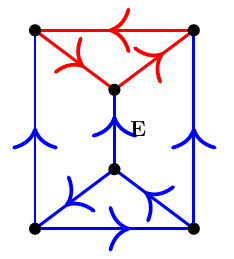
\includegraphics[scale=0.3]{img/restricted_ncl_1.png}
            \caption{Restricted NCL instance.}
            \label{fig:ps}
        \end{figure}
   \end{column}
   
\end{columns}   
\end{frame}

\begin{frame}{Nondeterministic Constraint Logic}
\begin{block}{Configuration-to-edge for Restricted NCL.}
    \begin{block}{Theorem (E.Demaine \& R.Hearn)}
    CONFIGURATION-TO-EDGE for restricted NCL is PSPACE-complete \cite{hearn_demaine_ncl_book}.
    \end{block}
        \begin{figure}
                \centering
                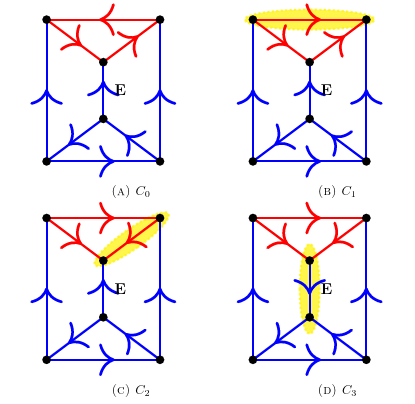
\includegraphics[scale=0.33]{img/restricted_ncl.png}
                \caption{Reconfiguration sequence reversing edge $E$.}
                \label{fig:ps}
        \end{figure}
    \end{block}

\end{frame}
